% questions.tex —— 2009 年·全国大纲卷Ⅰ·文科 · 题目内容片段（无答案）
% 由 tools/generate_projects.py 依来源总账自 2009/2009_数学真题_全国1文_试题.md 生成，勿手改（改源 MD 后重跑）


\gkpart{数学}

\begin{gktip}
\textbf{来源说明}：本题面依据固定源 PDF 两页 A3 题面逐题转录，原卷印刷页码 509–510。固定源不附答案，答案和解析均由本库独立复算。

\textbf{图形说明}：第 20、23 题的原卷图形关系重绘为 TikZ/PGFPlots 矢量图。图形标记所指的 PNG 不随仓库保存。
\end{gktip}

\gkpart{一、选择题}

\begin{question}
\gkti{1}$\sin585^\circ$ 的值为\mbox{（　　）}

（A）$-\dfrac{\sqrt2}{2}$\quad（B）$\dfrac{\sqrt2}{2}$\quad（C）$-\dfrac{\sqrt3}{2}$\quad（D）$\dfrac{\sqrt3}{2}$

\end{question}
\begin{question}
\gkti{2}设集合 $A=\{4,5,7,9\}$，$B=\{3,4,7,8,9\}$，全集 $U=A\cup B$，则集合 $\complement_U(A\cap B)$ 中的元素共有\mbox{（　　）}

（A）$3$ 个\quad（B）$4$ 个\quad（C）$5$ 个\quad（D）$6$ 个

\end{question}
\begin{question}
\gkti{3}不等式 $\left|\dfrac{x+1}{x-1}\right|<1$ 的解集为\mbox{（　　）}

（A）$\{x\mid0<x<1\}\cup\{x\mid x>1\}$\quad（B）$\{x\mid0<x<1\}$\quad（C）$\{x\mid-1<x<0\}$\quad（D）$\{x\mid x<0\}$

\end{question}
\begin{question}
\gkti{4}已知 $\tan\alpha=4$，$\cot\beta=\dfrac13$，则 $\tan(\alpha+\beta)=$\mbox{（　　）}

（A）$\dfrac7{11}$\quad（B）$-\dfrac7{11}$\quad（C）$\dfrac7{13}$\quad（D）$-\dfrac7{13}$

\end{question}
\begin{question}
\gkti{5}设双曲线 $\dfrac{x^2}{a^2}-\dfrac{y^2}{b^2}=1$（$a>0,b>0$）的渐近线与抛物线 $y=x^2+1$ 相切，则该双曲线的离心率等于\mbox{（　　）}

（A）$\sqrt3$\quad（B）$2$\quad（C）$\sqrt5$\quad（D）$\sqrt6$

\end{question}
\begin{question}
\gkti{6}已知函数 $f(x)$ 的反函数为 $g(x)=1+2\lg x$（$x>0$），则 $f(1)+g(1)=$\mbox{（　　）}

（A）$0$\quad（B）$1$\quad（C）$2$\quad（D）$4$

\end{question}
\begin{question}
\gkti{7}甲组有 $5$ 名男同学、$3$ 名女同学；乙组有 $6$ 名男同学、$2$ 名女同学。若从甲、乙两组中各选出 $2$ 名同学，则选出的 $4$ 人中恰有 $1$ 名女同学的不同选法共有\mbox{（　　）}

（A）$150$ 种\quad（B）$180$ 种\quad（C）$300$ 种\quad（D）$345$ 种

\end{question}
\begin{question}
\gkti{8}设非零向量 $\boldsymbol a,\boldsymbol b,\boldsymbol c$ 满足 $|\boldsymbol a|=|\boldsymbol b|=|\boldsymbol c|$，$\boldsymbol a+\boldsymbol b=\boldsymbol c$，则 $\langle\boldsymbol a,\boldsymbol b\rangle=$\mbox{（　　）}

（A）$150^\circ$\quad（B）$120^\circ$\quad（C）$60^\circ$\quad（D）$30^\circ$

\end{question}
\begin{question}
\gkti{9}已知三棱柱 $ABC-A_1B_1C_1$ 的侧棱与底面边长都相等，$A_1$ 在底面 $ABC$ 上的射影为 $BC$ 的中点，则异面直线 $AB$ 与 $CC_1$ 所成的角的余弦值为\mbox{（　　）}

（A）$\dfrac{\sqrt3}{4}$\quad（B）$\dfrac{\sqrt5}{4}$\quad（C）$\dfrac{\sqrt7}{4}$\quad（D）$\dfrac34$

\end{question}
\begin{question}
\gkti{10}如果函数 $y=3\cos(2x+\varphi)$ 的图象关于点 $\left(\dfrac{4\pi}{3},0\right)$ 中心对称，那么 $|\varphi|$ 的最小值为\mbox{（　　）}

（A）$\dfrac\pi6$\quad（B）$\dfrac\pi4$\quad（C）$\dfrac\pi3$\quad（D）$\dfrac\pi2$

\end{question}
\begin{question}
\gkti{11}已知二面角 $\alpha-l-\beta$ 为 $60^\circ$，动点 $P\text{、}Q$ 分别在面 $\alpha\text{、}\beta$ 内，$P$ 到 $\beta$ 的距离为 $\sqrt3$，$Q$ 到 $\alpha$ 的距离为 $2\sqrt3$，则 $P\text{、}Q$ 两点之间距离的最小值为\mbox{（　　）}

（A）$\sqrt2$\quad（B）$2$\quad（C）$2\sqrt3$\quad（D）$4$

\end{question}
\begin{question}
\gkti{12}已知椭圆 $C:\dfrac{x^2}{2}+y^2=1$ 的右焦点为 $F$，右准线为 $l$，点 $A\in l$，线段 $AF$ 交 $C$ 于点 $B$。若 $\overrightarrow{FA}=3\overrightarrow{FB}$，则 $|\overrightarrow{AF}|=$\mbox{（　　）}

（A）$\sqrt2$\quad（B）$2$\quad（C）$\sqrt3$\quad（D）$3$

\end{question}
\begin{question}
\gkti{13}已知椭圆 $C:\dfrac{x^2}{2}+y^2=1$ 的右焦点为 $F$，右准线为 $l$，点 $A\in l$，线段 $AF$ 交 $C$ 于点 $B$。若 $\overrightarrow{FA}=3\overrightarrow{FB}$，则 $|\overrightarrow{AF}|=$\mbox{（　　）}

（A）$\sqrt2$\quad（B）$2$\quad（C）$\sqrt3$\quad（D）$3$

\begin{gktip}
\textbf{固定源说明}：固定源 PDF 中第 12、13 题的题干和选项逐字相同，暂按原样保留，待取得同版勘误或其他可靠版本后核对。
\end{gktip}

\end{question}
\gkpart{二、填空题}

\begin{question}
\gkti{14}$(x-y)^{10}$ 的展开式中，$x^7y^3$ 的系数与 $x^3y^7$ 的系数之和等于\gkblank{}。

\end{question}
\begin{question}
\gkti{15}设等差数列 $\{a_n\}$ 的前 $n$ 项和为 $S_n$，若 $S_9=72$，则 $a_2+a_4+a_9=$\gkblank{}。

\end{question}
\begin{question}
\gkti{16}已知 $OA$ 为球 $O$ 的半径，过 $OA$ 的中点 $M$ 且垂直于 $OA$ 的平面截球面得到圆 $M$。若圆 $M$ 的面积为 $3\pi$，则球 $O$ 的表面积等于\gkblank{}。

\end{question}
\begin{question}
\gkti{17}若直线 $m$ 被两平行线 $l_1:x-y+1=0$ 与 $l_2:x-y+3=0$ 所截得的线段的长为 $2\sqrt2$，则 $m$ 的倾斜角可以是

① $15^\circ$　② $30^\circ$　③ $45^\circ$　④ $60^\circ$　⑤ $75^\circ$

其中正确答案的序号是\gkblank{}。（写出所有正确答案的序号）

\end{question}
\gkpart{三、解答题}

\begin{question}
\gkti{18}设等差数列 $\{a_n\}$ 的前 $n$ 项和为 $S_n$，公比是正数的等比数列 $\{b_n\}$ 的前 $n$ 项和为 $T_n$，已知 $a_1=1$，$b_1=3$，$a_3+b_3=17$，$T_3-S_3=12$，求 $\{a_n\}$、$\{b_n\}$ 的通项公式。

\end{question}
\begin{question}
\gkti{19}在 $\triangle ABC$ 中，内角 $A\text{、}B\text{、}C$ 的对边长分别为 $a\text{、}b\text{、}c$，已知 $a^2-c^2=2b$，且 $\sin B=4\cos A\sin C$，求 $b$。

\Needspace{0.4\textheight}
\end{question}
\begin{question}
\gkti{20}如图，四棱锥 $S-ABCD$ 中，底面 $ABCD$ 为矩形，$SD\perp$ 底面 $ABCD$，$AD=\sqrt2$，$DC=SD=2$，点 $M$ 在侧棱 $SC$ 上，$\angle ABM=60^\circ$。
\nopagebreak[4]
\begin{center}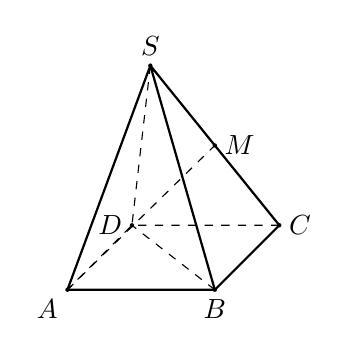
\begin{tikzpicture}[scale=.78,>=stealth]
\coordinate (A) at (0,0); \coordinate (B) at (2.4,0);
\coordinate (C) at (3.45,1.05); \coordinate (D) at (1.05,1.05);
\coordinate (S) at (1.35,3.65); \coordinate (M) at (2.40,2.35);
\draw[thick] (A)--(B)--(C);
\draw[dashed] (C)--(D)--(A) (S)--(D);
\draw[thick] (S)--(A) (S)--(B) (S)--(C);
\draw[dashed] (A)--(M) (B)--(D);
\fill (A) circle (1pt) node[below left] {$A$};
\fill (B) circle (1pt) node[below] {$B$};
\fill (C) circle (1pt) node[right] {$C$};
\fill (D) circle (1pt) node[left] {$D$};
\fill (S) circle (1pt) node[above] {$S$};
\fill (M) circle (1pt) node[right] {$M$};
\end{tikzpicture}
\end{center}
\nopagebreak[4]
（1） 证明：$M$ 是侧棱 $SC$ 的中点；

（2） 求二面角 $S-AM-B$ 的大小。

\end{question}
\begin{question}
\gkti{21}甲、乙二人进行一次围棋比赛，约定先胜 $3$ 局者获得这次比赛的胜利，比赛结束。假设在一局中，甲获胜的概率为 $0.6$，乙获胜的概率为 $0.4$，各局比赛结果相互独立，已知前 $2$ 局中甲、乙各胜 $1$ 局。

（1） 求再赛 $2$ 局结束这次比赛的概率；

（2） 求甲获得这次比赛胜利的概率。

\end{question}
\begin{question}
\gkti{22}已知函数 $f(x)=x^4-3x^2+6$。

（1） 讨论 $f(x)$ 的单调性；

（2） 设点 $P$ 在曲线 $y=f(x)$ 上，若该曲线在点 $P$ 处的切线 $l$ 通过坐标原点，求 $l$ 的方程。

\Needspace{0.4\textheight}
\end{question}
\begin{question}
\gkti{23}如图，已知抛物线 $E:y^2=x$ 与圆 $M:(x-4)^2+y^2=r^2$（$r>0$）相交于 $A\text{、}B\text{、}C\text{、}D$ 四个点。
\nopagebreak[4]
\begin{center}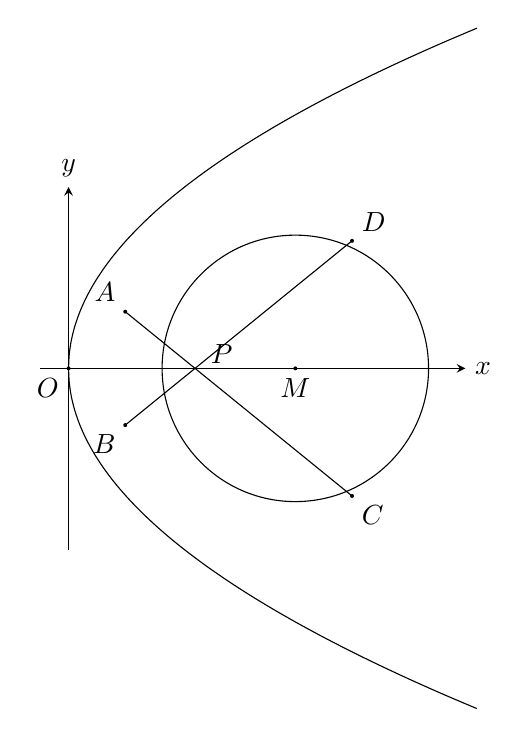
\begin{tikzpicture}[scale=.72,>=stealth]
\draw[->] (-.5,0)--(7,0) node[right] {$x$};
\draw[->] (0,-3.2)--(0,3.2) node[above] {$y$};
\draw[domain=0:6,smooth,variable=\x] plot ({\x*\x/5},{\x});
\draw[domain=0:6,smooth,variable=\x] plot ({\x*\x/5},{-\x});
\draw (4,0) circle (2.35);
\coordinate (A) at (1.0,1.0); \coordinate (B) at (1.0,-1.0);
\coordinate (C) at (5.0,-2.25); \coordinate (D) at (5.0,2.25);
\draw (A)--(C) (B)--(D);
\fill (0,0) circle (1pt) node[below left] {$O$};
\fill (4,0) circle (1pt) node[below] {$M$};
\fill (A) circle (1pt) node[above left] {$A$};
\fill (B) circle (1pt) node[below left] {$B$};
\fill (C) circle (1pt) node[below right] {$C$};
\fill (D) circle (1pt) node[above right] {$D$};
\node at (2.7,.25) {$P$};
\end{tikzpicture}
\end{center}
\nopagebreak[4]
（1） 求 $r$ 的取值范围；

（2） 当四边形 $ABCD$ 的面积最大时，求对角线 $AC\text{、}BD$ 的交点 $P$ 坐标。

\end{question}